\documentclass[11pt]{article}

\usepackage{url}
\usepackage{multicol}
\usepackage[english]{babel}
\usepackage[margin=1in]{geometry}
\usepackage{graphicx}
\usepackage{subcaption}
\usepackage{enumitem}
\usepackage{amsmath}
\usepackage{amssymb}
\usepackage{wasysym}
\usepackage{color}
\usepackage{float}
\usepackage{nomencl}
\usepackage[title]{appendix}
\makenomenclature
\usepackage{pdfpages}
\usepackage{algorithm}
\usepackage{algpseudocode}
\usepackage{hyperref}
\hypersetup{
    colorlinks=true,
    linkcolor=blue,
    filecolor=magenta,      
    urlcolor=cyan,
    pdftitle={Overleaf Example},
    pdfpagemode=FullScreen,
    }
\title{16-745 Optimal Control Lecture 1}
\author{Reid Graves} 

\begin{document}
\maketitle

\section{Crash Course in Dynamics}

\subsection{Continuous Time dynamics}
\begin{itemize}
    \item The most generic/general for a smooth system: Smooth meaning that there is not contact/impact such as a foot hitting the ground:
    \begin{align*}
        \dot{x} &= f(x,u) 
    \end{align*}
    Where $f$ is the dynamics, $x\in \mathbb{R}^n$ is the state, $u\in \mathbb{R}^m$ is the input, and $\dot{x}$ is the time derivative of the state.
    \item For a mechanical system:
    \begin{align*}
        x &= \begin{bmatrix}
            q \\
            v
        \end{bmatrix}
    \end{align*}
    Where $q$ is the configuration/pose, and is not always a vector, but can be something weirder than that, such as orientation in a rigid body. Attitude is not a vector, so roll and pitch are not a vector, but a weird group thing or manifold- will cover later. $v$ is the velocity, and is always a vector. So this is what the state vector is: Everything you need to specify the initial conditions of the system. 
\end{itemize}

\subsubsection{Pendulum Example}
% put the drawing here~~~~~~~~~~~~~~~~~~~~~~~~~~~~~~~~~~~~~~~~~~
\begin{figure}[H]
    \centering
    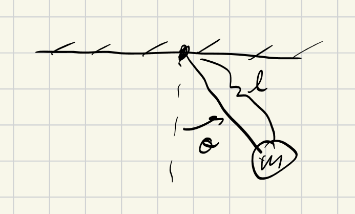
\includegraphics[width=0.5\linewidth]{lecture_1_1.png}
    \caption{pendulum example}
    \label{pendulum}
\end{figure}
Dynamics:
\begin{align*}
    ml^2\Ddot{\theta} + myl\sin(\theta) &= \tau
    \\
    q = \theta, \quad v = \Ddot{\theta}, \quad u&=\tau
    \\
    x &= \begin{bmatrix}
        \theta \\
        \dot{\theta}
    \end{bmatrix}
    \\
    \dot{x} &= \begin{bmatrix}
        \dot{\theta} \\
        \Ddot{\theta}
    \end{bmatrix}
 =
 \begin{bmatrix}
     \dot{\theta} \\
     \frac{-q}{l}\sin(\theta)+\frac{1}{ml^2}u
 \end{bmatrix}
\end{align*}
$q\in S^1$ (circle), $x\in S^1\times \mathbb{R}$ 

\subsection{Control-Affine Systems}
Still non-linear systems in general have term:
\begin{align*}
    \dot{x} &= f_0{x} + B(x)u
\end{align*}
Ax + B is affine- linear + constant. If you freeze x, then you have control affine system. Where $f_0(x)$ is drift, and $B(x)u$ is input jacobian. 
\begin{itemize}
    \item Most systems can be put in this form. For the pendulum:
    \begin{align*}
        f_0(x) &= \begin{bmatrix}
            \dot{\theta} \\
            \frac{-q}{l}\sin(\theta)
        \end{bmatrix}
            \\
            B(x) &= \begin{bmatrix}
                0 \\
                \frac{1}{ml^2}
            \end{bmatrix}
    \end{align*}
    \item If B is full rank, can pretty do anything you want with the system
\end{itemize}

\subsection{Manipulator Dynamics}
\begin{align*}
    M(q)\dot{v} + C(q,v) &= B(q)u + F
\end{align*}
$M$ term is mass matrix, $C$ term is dynamic bias (coriolis + gravity), $B$ is input jacobian, and $F$ is external forces
\begin{align*}
    \dot{q} &= G(q)v
\end{align*}
Call this equation the velocity kinematics. Can easily turn into:
\begin{align*}
    \dot{x} &= f(x,u) = \begin{bmatrix}
        G(q)v \\
        M^{-1}(q)(B(q)u + F-C)
    \end{bmatrix}
\end{align*}
\begin{itemize}
    \item Pendulum
\begin{align*}
    M(q) &= ml^2, \quad(q,v) = mgl\sin(\theta), B=I, G=I)
\end{align*}
\item All mechanical systems can be written this way
\item This is just a way of re-writing the Euler-Lagrange equation for:
\begin{align*}
    L &= \frac{1}{2} V^TM(q)V - U(q)
\end{align*}
Where first term is kinetic energy, second is potential energy. $M$ has some requirements, it corresponds to a mass written in joint space coordinates, so it is in quadratic form, and needs to be symmetric-positive-definite, i.e. must be invertable. 
\end{itemize}

\subsection{Linear Systems}
\begin{align*}
    \dot{x} &= A(t)x + B(t)u
\end{align*}
\begin{itemize}
    \item Called "time invariant" if $A(t) = A$, $B(t)=B$
    \item Called "time varying" otherwise
    \item Super important in control
    \item We often approximate non-linear systems with linear ones locally.
    \begin{align*}
        \dot{x} &= f(x,u) 
        \\
        A &= \frac{\partial f}{\partial x} \quad B = \frac{\partial f}{\partial u}
    \end{align*}
\end{itemize}






\end{document}
